% This document is based on a template created by Ted Pavlic (http://www.tedpavlic.com)


%----------------------------------------------------------------------------------------
%	PACKAGES AND OTHER DOCUMENT CONFIGURATIONS
%----------------------------------------------------------------------------------------

\documentclass{article}

\usepackage{fancyhdr} % Required for custom headers
\usepackage{lastpage} % Required to determine the last page for the footer
\usepackage{extramarks} % Required for headers and footers
\usepackage[usenames,dvipsnames]{color} % Required for custom colors
\usepackage{graphicx} % Required to insert images
\usepackage{subcaption}
\usepackage{listings} % Required for insertion of code
\usepackage{courier} % Required for the courier font
%\usepackage{lipsum} % Used for inserting dummy 'Lorem ipsum' text into the template
\usepackage{amsmath,physics,siunitx,amssymb}
\usepackage{placeins}
\usepackage{minted}
\usepackage{enumitem}
\usepackage{hyperref,cleveref}

% Margins
\topmargin=-0.45in
\evensidemargin=0in
\oddsidemargin=0in
\textwidth=6.5in
\textheight=9.0in
\headsep=0.25in

\linespread{1.1} % Line spacing

% Set up the header and footer
\pagestyle{fancy}
\lhead{\hmwkAuthorName} % Top left header
\chead{\hmwkClass\ (\hmwkClassTime): \hmwkTitle} % Top center head
%\rhead{\firstxmark} % Top right header
\lfoot{\lastxmark} % Bottom left footer
\cfoot{} % Bottom center footer
\rfoot{Page\ \thepage\ of\ \protect\pageref{LastPage}} % Bottom right footer
\renewcommand\headrulewidth{0.4pt} % Size of the header rule
\renewcommand\footrulewidth{0.4pt} % Size of the footer rule

\DeclareMathOperator*{\argmax}{arg\,max}

%\setlength\parindent{0pt} % Removes all indentation from paragraphs

%----------------------------------------------------------------------------------------
%	DOCUMENT STRUCTURE COMMANDS
%	Skip this unless you know what you're doing
%----------------------------------------------------------------------------------------

% Header and footer for when a page split occurs within a problem environment
\newcommand{\enterproblemHeader}[1]{
%\nobreak\extramarks{#1}{#1 continued on next page\ldots}\nobreak
%\nobreak\extramarks{#1 (continued)}{#1 continued on next page\ldots}\nobreak
}

% Header and footer for when a page split occurs between problem environments
\newcommand{\exitproblemHeader}[1]{
%\nobreak\extramarks{#1 (continued)}{#1 continued on next page\ldots}\nobreak
%\nobreak\extramarks{#1}{}\nobreak
}

\setcounter{secnumdepth}{0} % Removes default section numbers
\newcounter{problem} % Creates a counter to keep track of the number of problems
\setcounter{problem}{-1}

\newcommand{\problemName}{}
\newenvironment{problem}[1][Part \theproblem]{ % Makes a new environment called problem which takes 1 argument (custom name) but the default is "problem #"
	\stepcounter{problem} % Increase counter for number of problems
	\renewcommand{\problemName}{#1} % Assign \problemName the name of the problem
	\section{\problemName} % Make a section in the document with the custom problem count
	\enterproblemHeader{\problemName} % Header and footer within the environment
}{
	\exitproblemHeader{\problemName} % Header and footer after the environment
}

\newcommand{\problemAnswer}[1]{ % Defines the problem answer command with the content as the only argument
	\noindent\framebox[\columnwidth][c]{\begin{minipage}{0.98\columnwidth}#1\end{minipage}} % Makes the box around the problem answer and puts the content inside
}

\newcounter{subproblem}[problem]
\newcommand{\subproblemName}{}
\newenvironment{subproblem}[1][\theproblem~(\alph{subproblem})]{ % New environment for sections within  problems, takes 1 argument - the name of the section
	\stepcounter{subproblem}
	\renewcommand{\subproblemName}{#1} % Assign \problemName the name of the problem
	\subsection{\subproblemName} % Make a section in the document with the custom problem count
	\enterproblemHeader{\subproblemName} % Header and footer within the environment
}{
	\enterproblemHeader{\problemName} % Header and footer after the environment
}

\newcommand{\numberthis}{\addtocounter{equation}{1}\tag{\theequation}}

%----------------------------------------------------------------------------------------
%	NAME AND CLASS SECTION
%----------------------------------------------------------------------------------------

\newcommand{\hmwkTitle}{Assignment\ \#$3$} % Assignment title
\newcommand{\hmwkDueDate}{Monday,\ March\ 19,\ 2018} % Due date
\newcommand{\hmwkClass}{CSC411} % Course/class
\newcommand{\hmwkClassTime}{L2001} % Class/lecture time
\newcommand{\hmwkAuthorName}{Lukas Zhornyak} % Your name

%----------------------------------------------------------------------------------------
%	TITLE PAGE
%----------------------------------------------------------------------------------------

\title{
	\vspace{2in}
	\textmd{\textbf{\hmwkClass:\ \hmwkTitle}}\\
	\normalsize\vspace{0.1in}\small{Due\ on\ \hmwkDueDate}\\
	\vspace{0.1in}
	\vspace{3in}
}

\author{\textbf{\hmwkAuthorName}}
%\date{} % Insert date here if you want it to appear below your name

%----------------------------------------------------------------------------------------

\begin{document}

\maketitle
\clearpage

%----------------------------------------------------------------------------------------
%	ENVIRONMENT
%----------------------------------------------------------------------------------------

\begin{problem}[Environment]	
	Parts 1-6 were created with Python 2.7.14 with numpy 1.14.0, scipy 1.0.0, scikit-image 0.13.1, and matplotlib 2.1.1, as well as all associated dependencies. 
\end{problem}
\clearpage

%----------------------------------------------------------------------------------------
%	PART 1
%----------------------------------------------------------------------------------------
\FloatBarrier
\begin{problem}
	
	The headline dataset consists of two distinct parts: a set of "real" headlines and a set of "fake" headlines. There are 1968 real headlines, averaging 8.33 words per headline and 5.29 characters per word, and 1298 fake headlines, averaging 12.15 words per headline and 4.98 characters per word. Note that fake headlines seem to be longer but use smaller words, suggesting a difference in the language used in both sets. This gives credence to the feasibility of classifying a headline as fake or not based on the words used. Of course, just a headline is not very much information to go on, so it is likely that the accuracy will not be phenomenal.
	
	Some words that might prove useful in identifying a certain headline as fake or not are "says" (178 occurrences in the real data set vs 47 occurrences in the fake data set), "donald" (829 vs 228), and "hillary" (24 vs 159). The code used to obtain these words is given in the submitted code.
	
\end{problem}
\clearpage

%----------------------------------------------------------------------------------------
%	PART 2
%----------------------------------------------------------------------------------------

\begin{problem}
	
	To implement a Naive Bayes classifier, the ratio of the probability of a certain headline being fake to the ratio of it being real was examined when attempting to classify the headline:
	\begin{equation*}
		\frac{P(y = c \mid x_1, x_2, ..., x_p)}{P(y = c' \mid x_1, x_2, ..., x_p)} = \frac{P(y = c))\prod_{i=1}^{p}P(x_i \mid y = c)}{P(y = c')\prod_{i=1}^{p}P(x_i \mid y = c')}
	\end{equation*}
	where \(y\) is the label, \(x_i\) is a binary value indicating the presence of \(i\)-th keyword, \(p\) is the number of keywords, and \(c\) is the fake or real class, with \(c'\) being the opposite. If this value is larger then \(1\), \(P(y = c \mid x_1, x_2, ..., x_p)\) is larger than \(P(y = c' \mid x_1, x_2, ..., x_p)\) and thus the headline is classified as fake, and vice versa. Some minor preprocessing was done to convert the headlines into this one-hot feature representation.
	
	The above equation involves the product of several thousand different probabilities, many quite small. To prevent the issue of arithmetic underflow, the log of this probability ratio was used instead:
	\begin{equation*}
		\log \frac{P(y = c \mid x_1, x_2, ..., x_p)}{P(y = c' \mid x_1, x_2, ..., x_p)} = \log \frac{P(y = c)}{P(y = c')} + \sum_{i=1}^{p} \log \frac{P(x_i \mid y = c)}{P(x_i \mid y = c')}
	\end{equation*}
	as suggested in the handout. In this new formulation, a value greater than 0 denotes fake news. From this point, standard Naive Bayes was used to determine the probabilities.
	
	To tune the prior \(m\) and \(\hat{p}\), a basic gradient descent was performed on the validation set with initial values \(\hat{p} = 0.5\) and \(m = 10\). A secant approximation with small step size was used to approximate the gradient at each point. This resulted in small but consistent performance improvements of about 2 to 4 percent on the validation and testing set, but a loss in performance on the training set of about 1 to 3 percent. This suggests that this method is working properly to prevent over-fitting. The final accuracy achieved on the training and test sets was 0.9528 and 0.8408, respectively.
	
\end{problem}
\clearpage

%----------------------------------------------------------------------------------------
%	PART 3
%----------------------------------------------------------------------------------------

\FloatBarrier
\begin{problem}
	
	\begin{subproblem}
		To find the words that maximizes the probability that a given text is real or fake given the presence or absence of it, Bayes' rule can be applied:
		\begin{equation*}
			\argmax \limits_{i} P(y = c \mid x_i = a) = \argmax \limits_{i} \frac{P(x_i = a \mid y = c)P(y = c)}{P(x_i = a)}
		\end{equation*}
		where \(a\) is either 0 or 1, depending on whether the presence or absence is desired. Unfortunately, the true value of \(P(x_i = a)\) is not known very well and may often be 0 if only the dataset is used to determine it, so this formula cannot be applied as is. However, considering that only the ordering of the probabilities \(P(y = c \mid x_i)\) is needed to find the maximum and knowing that \(P(y = c' \mid x_i = a) = 1 - P(y = c \mid x_i = a)\), the maximizing \(x_i\) can also be found as
		\begin{align*}
			\argmax \limits_{i} P(y = c \mid x_i = a) &= \argmax \limits_{i} \frac{P(y = c \mid x_i = a)}{P(y = c' \mid x_i = a)}\\
			&= \argmax \limits_{i} \frac{P(x_i = a \mid y = c)P(y = c)}{P(x_i = a \mid y = c')P(y = c')} \\
			&= \argmax \limits_{i} \frac{P(x_i = a \mid y = c)}{P(x_i = a \mid y = c')} \\
			&= \argmax \limits_{i} \log(\frac{P(x_i = a \mid y = c)}{P(x_i = a \mid y = c')})
		\end{align*}
		where the log was added to assist in interpreting the value. If \(\log(\cdots)\) is greater than zero, it means that \(x_i = a\) predicts that the text has the label \(c\) and vice versa. Larger magnitudes indicate a greater probability. The top ten words and associated log probability ratios are shown in \cref{tab:q3a}. Note that the strength of the presence of a word in determining whether a headline is real or fake is significantly larger than the strength of its absence. This makes intuitive sense since a typical headline will not contain the majority of the words, regardless of it being fake or real.
		\begin{table}
			\begin{subtable}{0.25\linewidth}
				\centering
				\begin{tabular}{rS}
					ban           & 4.8711 \\
					korea         & 4.7235 \\
					travel        & 4.5503 \\
					turnbull      & 4.3693 \\
					australia     & 4.1123 \\
					tax           & 3.7654 \\
					paris         & 3.6560 \\
					james         & 3.5331 \\
					trumps        & 3.4768 \\
					debate        & 3.4654
				\end{tabular}
				\caption{Presence suggests real.}
			\end{subtable}%
			\begin{subtable}{0.25\linewidth}
				\centering
				\begin{tabular}{rS}
					trump         & 1.6880 \\
					the           & 0.2619 \\
					hillary       & 0.1040 \\
					a             & 0.0906 \\
					in            & 0.0869 \\
					to            & 0.0843 \\
					and           & 0.0787 \\
					is            & 0.0742 \\
					clinton       & 0.0735 \\
					for           & 0.0592
				\end{tabular}
			\caption{Absence suggests real.}
			\label{tab:3ab}
			\end{subtable}%
			\begin{subtable}{0.25\linewidth}
				\centering
				\begin{tabular}{rS}
					breaking      & 4.6573 \\
					3             & 4.4378 \\
					won           & 4.2343 \\
					soros         & 4.2343 \\
					u             & 4.0712 \\
					woman         & 4.0712 \\
					because       & 4.0712 \\
					homeless      & 4.0712 \\
					liberty       & 3.9785 \\
					reason        & 3.9785
				\end{tabular}
				\caption{Presence suggests fake.}
			\end{subtable}%
			\begin{subtable}{0.25\linewidth}
				\centering
				\begin{tabular}{rS}
					donald        & 0.3265 \\
					trumps        & 0.1204 \\ 
					us            & 0.0950 \\
					says          & 0.0507 \\
					ban           & 0.0425 \\
					north         & 0.0391 \\
					korea         & 0.0365 \\
					travel        & 0.0305 \\
					turnbull      & 0.0254 \\
					australia     & 0.0195
				\end{tabular}
				\caption{Absence suggests fake.}
			\end{subtable}
			\caption{Words most likely to denote a headline as real or fake based on its presence or absence with associated importance.}
			\label{tab:q3a}
		\end{table}
	\end{subproblem}

	\begin{subproblem}
		The top ten words, excluding stop words, and associated log probability ratios are shown in \cref{tab:q3b}.
		\begin{table}
			\begin{subtable}{0.25\linewidth}
				\centering
				\begin{tabular}{rS}
					ban           & 4.8711 \\
					korea         & 4.7235 \\
					travel        & 4.5503 \\
					turnbull      & 4.3693 \\
					australia     & 4.1123 \\
					tax           & 3.7654 \\
					paris         & 3.6560 \\
					james         & 3.5331 \\
					trumps        & 3.4768 \\
					debate        & 3.4654
				\end{tabular}
				\caption{Presence suggests real.}
			\end{subtable}%
			\begin{subtable}{0.25\linewidth}
				\centering
				\begin{tabular}{rS}	
					trump         & 1.6880 \\
					hillary       & 0.1040 \\
					clinton       & 0.0735 \\
					just          & 0.0532 \\
					america       & 0.0392 \\
					watch         & 0.0287 \\ 
					voter         & 0.0279 \\
					new           & 0.0265 \\
					victory       & 0.0257 \\
					voting        & 0.0249
				\end{tabular}
				\caption{Absence suggests real.}
				\label{tab:3bb}
			\end{subtable}%
			\begin{subtable}{0.25\linewidth}
				\centering
				\begin{tabular}{rS}
					breaking      & 4.6573 \\
					3             & 4.4378 \\
					won           & 4.2343 \\
					soros         & 4.2343 \\
					u             & 4.0712 \\
					woman         & 4.0712 \\
					homeless      & 4.0712 \\
					liberty       & 3.9785 \\
					reason        & 3.9785 \\
					7             & 3.8763
				\end{tabular}
				\caption{Presence suggests fake.}
			\end{subtable}%
			\begin{subtable}{0.25\linewidth}
				\centering
				\begin{tabular}{rS}
					donald        & 0.3265 \\
					trumps        & 0.1204 \\
					says          & 0.0507 \\
					ban           & 0.0425 \\
					north         & 0.0391 \\
					korea         & 0.0365 \\
					travel        & 0.0305 \\
					turnbull      & 0.0254 \\
					australia     & 0.0195 \\
					house         & 0.0188
				\end{tabular}
				\caption{Absence suggests fake.}
			\end{subtable}
			\caption{Words most likely to denote a headline as real or fake based on its presence or absence with associated importance, excluding stop words.}
			\label{tab:q3b}
		\end{table}
	\end{subproblem}

	\begin{subproblem}
		Stop words are present in all written works and normally do not carry with them any particular viewpoint or biases. Additionally, since there is a large number of them and since they are relatively common, slight differences in their prevalence in the trained data set may be exploited, potentially overfitting the data.
		
		From a different perspective, if there is a consistent difference in how stop words are used in real and fake headlines, then excluding these words causes a loss in information. Consider the difference in words present in \cref{tab:3ab,tab:3bb}. Almost all of the words in the original list are stop words and are not present in the second. This confirms an earlier observation made in part 1: fake headlines seem to use more but shorter words, suggesting a greater prevalence of linking words. 
	\end{subproblem}
	
\end{problem}
\clearpage

%----------------------------------------------------------------------------------------
%	PART 4
%----------------------------------------------------------------------------------------

\FloatBarrier
\begin{problem}
	
	A linear regression model was trained on the dataset using L2-regularization. The learning curve with cross-entropy loss is shown in \cref{fig:q4}, achieving a final accuracy of 0.8143 on the training set. The regularization term was selected by minimizing the validation error at the end of training using the minimize\_scalar function provided in scipy.optimize with the Brent algorithm. The resulted in the selection of an regularization weight of 0.000061.
	
	\begin{figure}
		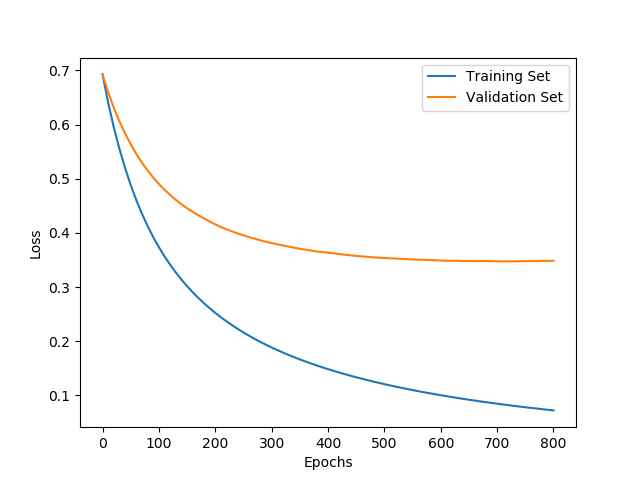
\includegraphics[width=\linewidth]{q4}
		\caption{Normalized loss for the training and validation sets for 800 epochs with a regularization term of 0.000061}
		\label{fig:q4}
	\end{figure}
	
\end{problem}
\clearpage

%----------------------------------------------------------------------------------------
%	PART 5
%----------------------------------------------------------------------------------------

\FloatBarrier
\begin{problem}
	
	In both formulations, \(I_i(x)\) denotes the selector function, choosing the \(i\)-th variable of the input vector \(x\). In the case of logistic regression, \(\theta_i\) are the parameters being directly optimized by the optimization procedure. For Naive Bayes, their meaning can be found by continuing the derivation started in part 2:
	
	\begin{align*}
		\log \frac{P(y = c \mid x_1, x_2, ..., x_p)}{P(y = c' \mid x_1, x_2, ..., x_p)} &= \log \frac{P(y = c)}{P(y = c')} + \sum_{i=1}^{p} \log \frac{P(x_i \mid y = c)}{P(x_i \mid y = c')} \\
		&= \log \frac{P(y = c)}{P(y = c')} + \sum_{i=1}^{p}\qty(\log \frac{P(x_i = 1 \mid y = c)}{P(x_i = 1 \mid y = c')}x_i + \log \frac{P(x_i = 0 \mid y = c)}{P(x_i = 0 \mid y = c')}(1 - x_i)) \\
		&= \qty(\log \frac{P(y = c)}{P(y = c')} + \sum_{i=1}^{p} \log \frac{P(x_i = 0 \mid y = c)}{P(x_i = 0 \mid y = c')}) + \\
		&\qquad\qquad \sum_{i=1}^{p}\qty(\log \frac{P(x_i = 1 \mid y = c)}{P(x_i = 1 \mid y = c')} - \log \frac{P(x_i = 0 \mid y = c)}{P(x_i = 0 \mid y = c')})x_i \\
		&= \theta_0 + \sum_{i=1}^{p} \theta_i x_i
	\end{align*}
	which is the form desired. Compare this with with the formulation obtained in part 3. Hence, in the case of Naive Bayes \(\theta_i\) represents the combination of the impact of the presence as well as the negation of the impact of its absence, normally present in the constant bias term. 
	
	For both logistic regression and naive bayes, the threshold is zero.
	
\end{problem}
\clearpage

%----------------------------------------------------------------------------------------
%	PART 6
%----------------------------------------------------------------------------------------

\FloatBarrier
\begin{problem}
	
	\begin{subproblem}
		
		Compared with \cref{tab:q3a}, the resulting parameters share only a couple of the same words, and not in the same order. These similarities suggest that both are generally looking for the same features to classify The larger differences are to be expected, however, since the parameters do not map directly to any of the probabilities in part 3. Instead, they in some sense represent the combination of both the presence of the words negation of its absence (normally accounted for in the constant bias). From a purely subjective perspective however, the words in each list match the same tone as those from before; more neutral, "reportive" words seem to suggest that a headline is real, while more emotional, aggressive, and idealistic terms are associated with it being fake.
		
		\begin{table}
			\begin{subtable}{0.5\linewidth}
				\centering
				\begin{tabular}{rS}	
					vandalised     & -1.2439 \\
					share          & -1.2043 \\
					business       & -1.2039 \\
					debate         & -1.1903 \\
					trumps         & -1.1848 \\
					australia      & -1.1791 \\
					keating        & -1.1749 \\
					affect         & -1.1667 \\
					speaks         & -1.1633 \\
					love           & -1.1324
				\end{tabular}
				\caption{Presence suggests real.}
			\end{subtable}%
			\begin{subtable}{0.5\linewidth}
				\centering
				\begin{tabular}{rS}
					information   & 1.3171 \\
					won           & 1.3162 \\
					go            & 1.3132 \\
					alt           & 1.2981 \\
					erase         & 1.2293 \\
					artificial    & 1.2283 \\
					reset         & 1.2230 \\
					breaking      & 1.1966 \\
					autistic      & 1.1911 \\
					entire        & 1.1858
				\end{tabular}
				\caption{Presence suggests fake.}
			\end{subtable}
			\caption{Words with largest and smallest associated parameters, signifying fake or real respectively.}
			\label{tab:q4a}
		\end{table}
	\end{subproblem}
	
	\begin{subproblem}
		
		As before, there is only slight similarity between \cref{tab:q3b,tab:q4b}. However, the removal of stop words seems to have resulted in less of a change in the words selected by logistic regression. This may be the result of the combination of both the presence and negating the absence, as mentioned before - stop words may not be very useful for actually predicting a headline as real or fake and could represent overfitting.
		
		\begin{table}
			\begin{subtable}{0.5\linewidth}
				\centering
				\begin{tabular}{rS}	
					vandalised     & -1.2439 \\
					share          & -1.2043 \\
					business       & -1.2039 \\
					debate         & -1.1903 \\
					trumps         & -1.1848 \\
					australia      & -1.1791 \\
					keating        & -1.1749 \\
					affect         & -1.1667 \\
					speaks         & -1.1633 \\
					love           & -1.1324
				\end{tabular}
				\caption{Presence suggests real.}
			\end{subtable}%
			\begin{subtable}{0.5\linewidth}
				\centering
				\begin{tabular}{rS}
					information   & 1.3171 \\
					won           & 1.3162 \\
					alt           & 1.2981 \\
					erase         & 1.2293 \\
					artificial    & 1.2283 \\
					reset         & 1.2230 \\
					breaking      & 1.1966 \\
					autistic      & 1.1911 \\
					entire        & 1.1858 \\
					display       & 1.1806
				\end{tabular}
				\caption{Presence suggests fake.}
			\end{subtable}
			\caption{Words, excluding stop words, with largest and smallest associated parameters, signifying fake or real respectively.}
			\label{tab:q4b}
		\end{table}
	\end{subproblem}
	
	\begin{subproblem}
		This is probably not a good idea in general since the relationship between the magnitude of the different inputs may not be well known. For example, if the input is not normalized and two variables, having differen magnitudes, each contribute about the same to determining the class of an input, then the variable with the larger value will necessarily have a smaller associated parameter. By only considering the largest parameters then, a skewed and potentially incorrect view on what is most important for classification may be developed. Even if the data is normalized, the means of the different variables may still vary. In this specific case however, the input is a binary signal. Thus, each parameter can be interpreted in the same context and thus comparing by magnitude is valid.
	\end{subproblem}
	
\end{problem}
\clearpage

%----------------------------------------------------------------------------------------
%	PART 7
%----------------------------------------------------------------------------------------
\FloatBarrier
\begin{problem}
	
	\begin{subproblem}
		A decision tree was trained on the data set with parameters \(\mathrm{max\_depth} = 100\), \(\mathrm{max\_features} = 1000\), \(\mathrm{criterion} = \mathrm{'gini'}\), \(\mathrm{splitter} = \mathrm{'best'}\), \(\mathrm{min\_samples\_leaf} = 1\), and  \(\mathrm{min\_samples\_split} = 5\). This achieved a final accuracy of 75.91\% on the testing set. A plot of the accuracy on the training and validation set versus the selection of the max\_depth is shown in \cref{fig:q7a}.
		
		The parameters above were selected by performing a grid search on the a predetermined set of reasonable values. The combinations of parameters that produced the largest accuracy on the validation set was selected as the best settings and saved.
		
		\begin{figure}
			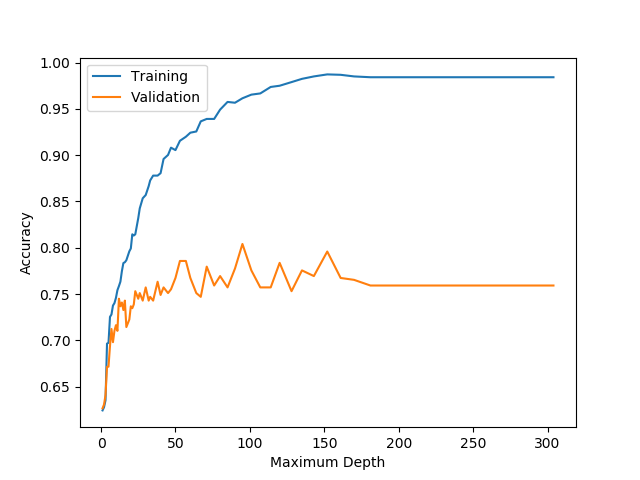
\includegraphics[width=\linewidth]{q7}
			\caption{Accuracy on the training and validation set versus the maximum depth of the decision tree.}
			\label{fig:q7a}
		\end{figure}
	\end{subproblem}
	
	\begin{subproblem}
		The first two layers of the decision tree are shown in \cref{fig:q7b}. The words present as upper level determination boundaries in this decision tree seem to share somewhat more in common with the words identified from naive bayes rather than logistic regression. Additionally, there are several unique words in these upper layers that do not appear in either previous set. These new words primarily seem to be classifying only a few words at a time; the words that separate the set into two large parts seem to generally overlap with those found previously.
		\begin{figure}
			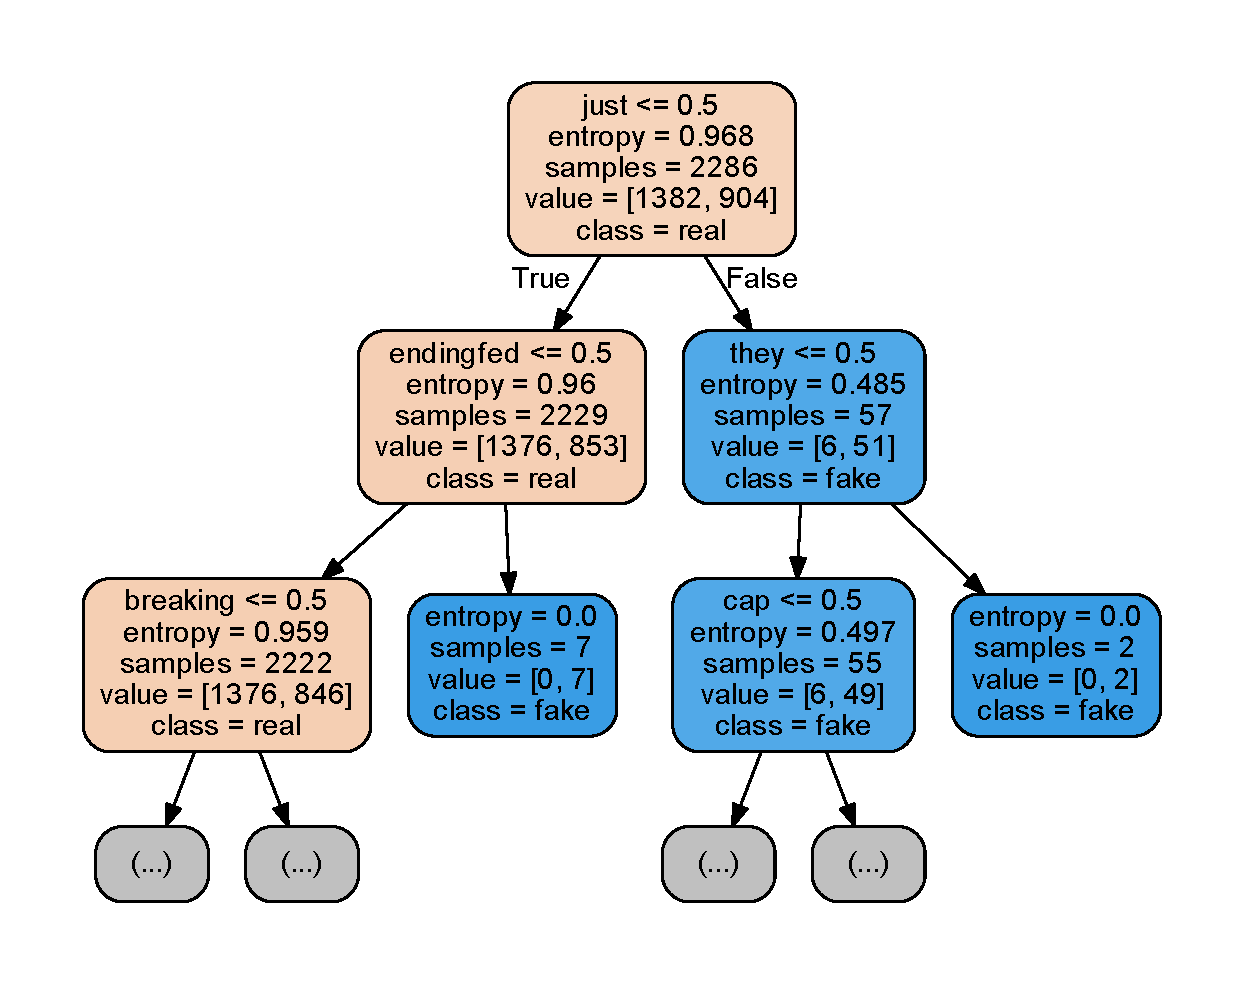
\includegraphics[width=\linewidth]{decision_tree}
			\caption{First two layers of the decision tree.}
			\label{fig:q7b}
		\end{figure}
	\end{subproblem}

	\begin{subproblem}
		The performance of each different classifier is summarised in \cref{tab:q7}. 
		
		The best performance outside of the training set was seen in the Naive Bayes model, beating the logistic regression model by about a percentage point. On the training set meanwhile, the best performance was achieved by the logistic regression model, achieving nearly perfect accuracy. This discrepancy suggests greater overfitting in the logistic model than the Naive Bayes model.
		
		The worst performance on the validation and testing sets was observed with the decision tree model. The worst performance in the training set was observed with the Naive Bayes model; however, this is likely the result of tuning the prior to maximize validation accuracy as opposed to training set accuracy.
		
		That decision tree model achieved the worst accuracy on the validation set and testing set despite very high accuracy on the training set suggests that this model overfit the data presented the most out of the three models. Additionally, the drop in accuracy from the validation set to the testing set suggests that there was some overfitting in the selection of hyper parameters. This matches what was observed - most values of the hyper parameters produced similar accuracy hence the difference in accuracy was likely due in part due to random chance in the data set.
		\begin{table}
			\centering
			\caption{Summary of the accuracy of the three different tested classification model on the training, validation, and testing set.}
			\label{tab:q7}
			\begin{tabular}{rSSS}
				& {Naive Bayes} & {Logistic Regression} & {Decision Tree} \\
				\hline
				Training & 0.9528 & 0.9947 & 0.9856 \\
				Validation & 0.8490 & 0.8327 & 0.8000  \\
				Testing & 0.8408 & 0.8327 & 0.7591 \\
				\hline
			\end{tabular}
		\end{table}
	\end{subproblem}
	
\end{problem}
\clearpage

%----------------------------------------------------------------------------------------
%	PART 8
%----------------------------------------------------------------------------------------

\FloatBarrier
\begin{problem}
	\begin{subproblem}
		The code used to calculate the mutual information given the index of a word is shown below.	For the first split of the decision tree (based on "just"), the calculated mutual information of the split is 0.020142.
		\begin{minted}[mathescape, linenos, numbersep=5pt, gobble=2, frame=lines, framesep=2mm, tabsize=4, breaklines]{python}
			def mutual_information_to_output(data, word):
				def entropy(a):
					pa = np.mean(a)
					return -pa * np.log2(pa) - (1 - pa) * np.log2(1 - pa)
			
				present = data[0].astype(bool)
				not_present = np.logical_not(present)
				label = data[1]
				
				# mean is equivalent to probability
				return entropy(label) - \
					np.mean(present) * entropy(label[present]) - \
					np.mean(not_present) * entropy(label[not_present])
		\end{minted}
	\end{subproblem}

	\begin{subproblem}
		For the randomly chosen word "fellowship", the calculated mutual information using the code above of a split based on the presence of this word is 0.000586. Given that the initial split will be applied to every headline, it is to be expected that the information gain of the initial split is larger than that of a randomly selected word. In further tests against nine other random words, all other words had an information gain less than or equal to the information gain of "fellowship".
		
		The word chosen for the initial split is not necessarily the word that has the largest information gain however. The information gain of a split based on the word "trumps", chosen because of its appearance in several of the list of most important words for Naive Bayes and logistic regression, is 0.046139. Despite this large information gain, it is likely that a split about "trumps" is not an optimal initial split because of its affect on later decisions; "just" is probably better in this regard, given that it was selected.
	\end{subproblem}
\end{problem}
\clearpage

%----------------------------------------------------------------------------------------

\end{document}